\documentclass{article}%
\usepackage[T1]{fontenc}%
\usepackage[utf8]{inputenc}%
\usepackage{lmodern}%
\usepackage{textcomp}%
\usepackage{lastpage}%
\usepackage[head=40pt,margin=0.5in,bottom=0.6in]{geometry}%
\usepackage{graphicx}%
%
\title{\textbf{Protestan en una parroquia de Charallave por tener cuatro días sin luz}}%
\author{El Nacional Web}%
\date{21/10/2018}%
%
\begin{document}%
\normalsize%
\maketitle%
\textbf{URL: }%
http://www.el{-}nacional.com/noticias/protestas/protestan{-}una{-}parroquia{-}charallave{-}por{-}tener{-}cuatro{-}dias{-}sin{-}luz\_256638\newline%
%
\textbf{Periodico: }%
EN, %
ID: %
256638, %
Seccion: %
Protestas\newline%
%
\textbf{Palabras Claves: }%
Luz, Corpoelec, Protestas, Gobierno\newline%
%
\textbf{Derecho: }%
2.8, %
Otros Derechos: %
, %
Sub Derechos: %
2.8.1\newline%
%
\textbf{EP: }%
SI\newline%
\newline%
%
\textbf{\textit{Los afectados denuncian que sus alimentos se han descompuesto~por la falta del servicio~}}%
\newline%
\newline%
%
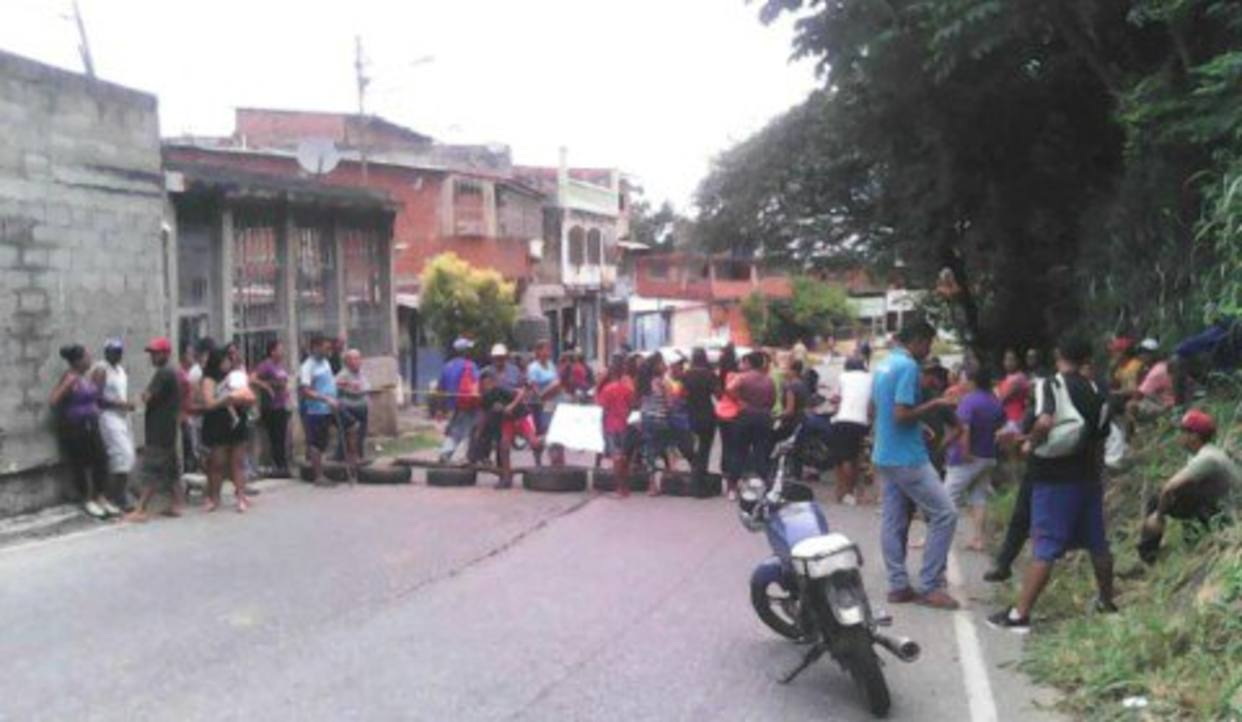
\includegraphics[width=300px]{68.jpg}%
\newline%
%
Habitantes de la parroquia Las Brisas de~Charallave, estado Miranda, protestan este domingo por no tener luz desde hace cuatro días.%
\newline%
%
Reportes de Twitter indican que desde el jueves 18 de septiembre no tienen el servicio eléctrico. Denuncian que los alimentos se les han descompuesto por la falta de energía.%
\newline%
%
En consecuencia, exigen respuesta y solución por parte Luis Motta Domínguez, ministro de Electricidad de Venezuela y de la Corporación Eléctrica Nacional (Corpoelec).%
\newline%
%
\end{document}